Consider the following call:

\t{label(5, 10, [0, 1, 1, 2], [1, 2, 3, 4])}

There are a total of $5$ stations, and $4$ links connecting pairs of stations with indices $(0, 1)$, $(1, 2)$, $(1, 3)$ and $(2, 4)$. Each label can be an integer from $0$ to $k=10$.

In order to report the following labelling:

\begin{center}
\renewcommand{\arraystretch}{1.5}
\begin{tabular}{|c|c|}
\hline
Index & Lable  \\
\hline
0 & 6 \\
\hline
1 & 2 \\
\hline
2 & 9 \\
\hline
3 & 3\\
\hline
4 & 7\\
\hline

\end{tabular}
\end{center}

the \t{label} procedure should return [$6$, $2$, $9$, $3$, $7$]. The numbers in the following figure show the indices (left panel) and assigned labels (right panel).

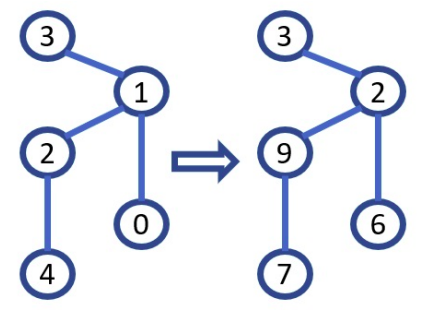
\includegraphics{1.png}

Assume the labels have been assigned as described above and consider the following call:

\t{find\_next\_station(9, 6, [2, 7])}

This means that the station holding the packet has label $9$, and the target station has label $6$. The labels of stations on the path to the target station are $[9, 2, 6]$. Hence, the call should return $2$, which is the label of the station that the packet should be forwarded to (which has index $1$).

Consider another possible call:

\t{find\_next\_station(2, 3, [3, 6, 9])}

The procedure should return $3$, since the target station with label $3$ is a neighbour of the station with
label $2$, and hence should receive the packet directly.
